\subsection{Chorus and Flanger Effect}

The chorus effect is obtained when a sound is delayed and then mixed with its original version. 
The chorus effect generator takes as an input a single audio signal and applies different delay values on it. Chorus effect can be applied using one delay. Each of the delayed signal are then mixed with original audio input. 
An \gls{lfo} (Low Frequency Oscillator) can be used to make the delay times vary. Different \gls{lfo}s can be used for each of the delay channels to make a richer sound mix and avoiding repetitive sound but it implies more computations. The same \gls{lfo} can be used for all the delay channels but not at the same cycle for each delay. \\

Different parameters can be changed to tune the chorus effect:\\
\begin{itemize}
\item \textbf{Delay time}: the time difference between the original sound and the delayed one.
\item \textbf{Chorus size}: the number of delayed sounds that will be mixed.
\item \textbf{Depth}: the amplitude of the of the modulation frequency.
\end{itemize}

The flanger effect is the same as the chorus effect but with shorter delay times.

A block diagram for  the chorus effect is shown in figure \autoref{fig:chorus_diag}.

\begin{figure} [htbp!]
	\centering
\begin{picture}(0,0)%
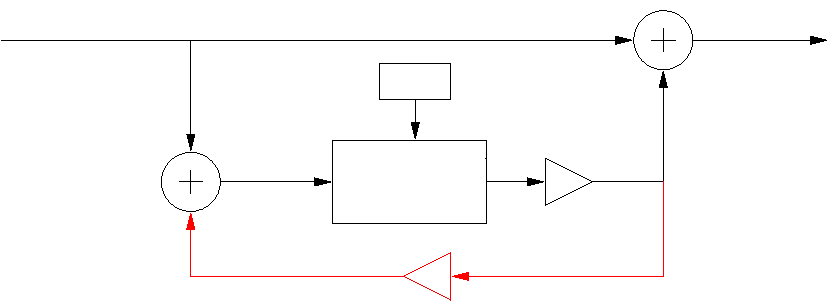
\includegraphics{chorus_diag.pdf}%
\end{picture}%
\setlength{\unitlength}{4144sp}%
%
\begingroup\makeatletter\ifx\SetFigFont\undefined%
\gdef\SetFigFont#1#2#3#4#5{%
  \reset@font\fontsize{#1}{#2pt}%
  \fontfamily{#3}\fontseries{#4}\fontshape{#5}%
  \selectfont}%
\fi\endgroup%
\begin{picture}(6327,1713)(3766,-2188)
\put(9406,-646){$Output$}%
\put(6706,-1186){$LFO$}%
\put(6436,-1906){$Delay$}%
\put(8101,-1636){$Gain$}%
\put(3781,-646){$Input$}%
\end{picture}%

\caption{Block Diagram of the chorus effect.}
\label{fig:chorus_diag}
\end{figure}








